\section{Simplification Queries}
\label{sec:simplification-queries}

In this section, given a fixed polyline we design a datastructure that allows optimal simplification queries, i.e., for 
an input \(\varepsilon\) we find the smallest simplification within \(\varepsilon\). In total, we will be able to construct the datastructure in time \(\O(n^4\log n)\) and allow queries in time \(\O(\log n)\) where \(n\) is the length of the polyline.

\begin{lemma}\label{lem:datastructure-existence}
  Given a fixed polyline \(P\) of length \(n\). There is a datastructure \(D\) that uses \(\O(n^2)\) space that allows querying polyline simplifications in logarithmic time. That is, \(D\) allows queries of the following form: For \(\varepsilon > 0\) find the smallest simplification \(Q\) of \(P\) with \(\delta^F(P, Q) \leq \varepsilon\).
\end{lemma}

\begin{proof}
  The datastructure is a sorted array of length \(n\) with entries \((I, S_I)\) where \(I \subseteq \R_{\geq 0}\) and \(S_I\) is a simplification of \(P\). The \(I\) are intervals of the form \([\varepsilon_i, \varepsilon_{i+1})\) that partition \(\R_{\geq 0}\) with \(0 = \varepsilon_0 < \varepsilon_1 < \cdots < \varepsilon_{n} = \infty\) that satisfy the property that for all \(\varepsilon \in I\) the simplification size is the same and \(S_I\) is a simplification of that size with the smallest Fréchet distance. 

	Given an \(\varepsilon\) we can query for the simplification using binary search on this interval in time \(\O(\log(n))\) to lookup the simplification. By construction this simplification must be optimal.

	This datastructure needs to store \(\O(n)\) many intervals and simplifications and each simplification requires linear space resulting in \(\O(n^2)\) space consumption.
\end{proof}

This result is rather unspectacular as it does not give us any indication how to determine these intervals and thus how to construct the datastructure efficiently. Before we go into the construction, we mention that \cref{lem:datastructure-existence} did not make any assumption on how to measure the simplification against the polyline. Thus it also works in the local and Hausdorff cases albeit with different constructions than outlined here. 

\subsection{Datastructure Construction}
\label{ssec:ds-construction}

To construct the datastructure from \cref{lem:datastructure-existence}, it suffices to find the respective intervals as we can use them to query for the respective simplifications using any simplification algorithm. Thus the relevant information is the \(\varepsilon_i\) at which the simplification size changes.

These \(\varepsilon_i\) are independent of the simplification algorithm used, they only depend on the polyline. We analyze now the \citeauthor{on_optimal_polyline_simplification_using_the_hausdorff_and_frechet_distance} algorithm to identify all possible valus \(\varepsilon\) where the simplification size might change. We use the implicit algorithm as a basis as it is more obvious which \(\varepsilon\) need to be considered. Unlike previous sections, we adjust our notation for the equations solutions defined in \cref{sec:preliminaries} and for the relations defined in \cref{sec:implicit_polyline_simplification} to account for the \(\varepsilon\).

Using the implicit approach, we note that \(\varepsilon\) only appears in decision problems. More specifically in the following ones:
\begin{enumerate}
  \item During initialization (line 3 in \cref{algo:simplify_simple_implicit})
	\item During the Fréchet distance decision procedure (line 19 in \cref{algo:simplify_simple_implicit})
\end{enumerate}

The Fréchet distance decision procedure requires \(\varepsilon\) for the relations \(\overset e\rightarrow\) and \(\overset e\leftarrow\). In total, \(\varepsilon\) is only involved in decision problems thus we only need to track the values at which the value of each possible decision changes. 

For the initialization, there is at most one such changing event per point on the polyline as we only need to track if the point and all previous ones are within \(\varepsilon\) of the starting point. Thus, this gives us only linearly many events to consider.

The relation \(\leftrightarrow\) yields \(\O(n^3)\) many events \(\varepsilon\) to consider. We pick two points for the line segment and one to test against the line segment. For each such triple there is one \(\varepsilon\) at which the line segment is reachable from the point and for all larger \(\varepsilon\) it remains reachable. 

For the two relations \(\overset e\rightarrow\) and \(\overset e\leftarrow\) there are \(\O(n^4)\) many event types to consider: Pick two points for the line segment and two further points \(u\) and \(v\) to compare. We may assume that both \(u\) and \(v\) reach the line segment as we have already included all such reachability events. To get the total amount of events we need to determine how many events per line segment and pair of points there are. 

\begin{lemma}\label{lem:event_counts}
  Let \(e\) be a line segment and \(u\) and \(v\) be points. Let \(d\) be the dimension.
	\begin{enumerate}
		\item The solution set 
			\[S = \set{\varepsilon \mid t \in [0, 1], \varepsilon = \delta_2(e(t), u) = \delta_2(e(t), v)}\]
		is an interval \(I \subseteq \R_{\geq 0}\). Note that single points and the empty set are closed intervals.
			
		\item For \(\delta \in \set{\delta_1, \delta_\infty}\) the solution set 
			\[S = \set{\varepsilon \mid t \in [0, 1], \varepsilon = \delta(e(t), u) = \delta(e(t), v)}\]
		is the union of at most \(\O(d)\) many closed intervals. 	

		\item For \(\delta = \delta_\ell\) with \(\ell \in \N_{\geq 3}\) the solution set 
			\[S = \set{\varepsilon \mid t \in [0, 1], \varepsilon = \delta(e(t), u) = \delta(e(t), v)}\]
			is the union of \(\O(d \cdot \ell)\) many closed intervals. \(\O(\ell)\) many closed intervals suffice if \(\ell\) is even.
	\end{enumerate}
\end{lemma}

\begin{proof}
  \begin{enumerate}
		\item Consider the Voronoi diagram for the two points \(u\) and \(v\). The boundary between the two cells correspond to the points which are equidistant from both points and is a single line (or a hyperplane for general dimensions). The intersection of this boundary and the line segment is either empty, a single point or a line segment itself. The corresponding distances thus have one of the stated forms. 

		\item Define the function \(f(t) = \delta(e(t), u)\) and \(g(t) = \delta(e(t), v)\). For the Manhattan and Chebyshev distance both functions are piecewise linear convex functions. Each line segment of \(f\) can intersect \(g\) in at most two interval resulting in \(\O(d)\) many intervals. To show the last argument, note that liner functions are concave. Subtract the lienar function from \(g\) to obtain a new convex function whose zeros correspond to the intersections of the line and \(g\). A convex function cannot have three distjoint zeros.

		\item For even \(\ell\), \(\delta(e(t), u) = \delta(e(t),v)\) simplifies to a polynomial in \(t\) of degree \(\ell\) which ahs \(\O(\ell)\) many solutions which correspond to \(\O(\ell)\) many intervals. For the odd case, we combine this with the trick used to solve equations involving the Manhattan distance as described in \cref{sec:equation_solving}. We can partition the real numbers into \(\O(d)\) many intervals such that in each of these intervals the sides of the equation simplify to polynomials of degree \(\O(\ell)\). In total we get \(\O(d\ell)\) intervals at most. 
  \end{enumerate}
\end{proof}

To obtain all events, we need to find the \(\varepsilon\) where the result of the two relations changes. This happens exactly at the solution sets described in \cref{lem:event_counts}. To see this, we observe that the result of both relations can only change if the first solution of the first on the line segment crosses either the first solution of the second point (in the case of \(\overset e\rightarrow\)), or the second solution of the second point (in the case of \(\overset e\leftarrow\)). Thus, the relevant events occur when there is a point on the line segment that has distance exactly \(\varepsilon\)to both points. 

Single points are themselves events and for proper intervals we only need to include the boundaries. Thus the total amount of events depends on the distance function and dimension used. 

\begin{observation}\label{obs:event-count}
	The amount of events at which the simplification can change is 
	\begin{itemize}
		\item \(\O(n^4)\) when using the Euclidean distance, 
		\item \(\O((dn)^4)\) when using the Manhattan or Chebyshev distance,
		\item \(\O((\ell n)^4)\) when using an even \(\ell\)-Minkowski distance with \(\ell \geq 4\), or 
		\item \(\O((d \ell n)^4)\) when using an odd \(\ell\)-Minkowski distance
	\end{itemize}
\end{observation}

In the following we use the amount of events from the Euclidean case to analyze runtimes. We will state the total runtimes for the other cases at the end. 

Using \cref{obs:event-count} we can formulate a simple \(\O(n^7)\) algorithm to construct the datastructure: Compute all events, sort them and process them in order. For each, apply the cubic runtime algorithm and test if the simplification size changed. If so we have found the boundary of the current interval.

With a simple trick, we can reduce the runtime down to \(\O(n^4 \log n)\). After sorting the events, we perform binary search to find the events that constitute the boundaries of the intervals. We need to perform the binary search \(\O(n)\) times, once for each possible simplification size. Each binary search takes runtime \(\log(n^4) \in \O(\log n)\) resulting in \(\O(n \log n)\) many events to test. For each event we perform the cubic simplification algorithm to obtain \(\O(n^4 \log n)\) for this step. As both the sorting step and the search step require \(\O(n^4\log n)\) time, the total algorithm requires the same time. 

\begin{algorithm}[ht]
  \DontPrintSemicolon
  \KwData{Polyline \(P\) of length \(n\)}
  \KwResult{Sorted array of events}
  \BlankLine
	\(events \gets Array()\) \tcp{capacity can be bounded based on dimension and \(\delta\)}
	\For{\(i=1,\dots, d\)}{
		\(events.append(\delta(P(0), P(i)))\)
	}
	\For{\(0 \leq i < j \leq n, k = 0, \dots, n\)}{
		\(\varepsilon \gets \min_{t \in [0, 1]} \delta((1-t)P(i) + tP(j), P(k))\)\;
		\(events.append(\varepsilon)\)
	}
	\For{\(0 \leq i' < i \leq n, 0 \leq u < v \leq n\)}{
		Let \(S\) be the set of solutions in \((0,1)\) to \(\delta((1-t)P(i') + tP(i), P(u)) = \delta((1-t)P(i') + tP(i), P(v))\), 
		for interval solutions add only the boundaries \;
		\(events.addAll(S)\)
	}
	Sort \(events\) and filter out duplicates\;
  \caption{EventList(\(P\))}
  \label{algo:event-list}
\end{algorithm}

\begin{algorithm}[ht]
	\(events \gets EventList(P)\)\;
	\(D \gets Array(n)\)\;
	\(D[n-1] = (0, P)\)\;
	\For{\(i=n-1,\dots, 1\)}{
		\(left \gets 0, right \gets |events|\)\;
		\While{\(right - left > 1\)}{
			\(mid \gets \floor{\frac{left + right}{2}}\)\;
			\(k \gets \) Simplification size with \(\varepsilon = events[mid]\)\;
			\If{\(k < i\)}{
				\(right \gets mid\)
			}\ElseIf{\(k > i\)}{
				\(left \gets mid\)
			}\ElseIf{Simplification size with \(\varepsilon = events[mid-1]\) is \(i+1\)}{
				\(left \gets mid, right \gets mid + 1\)
			}\Else{
				\(right \gets mid\)
			}
		}
		\(\varepsilon \gets events[left]\)\;
		Compute a simplification \(S\) with \(\varepsilon\)\;
		\(D[i-1] = (\varepsilon, S)\)
	}
  \caption{QueryDatastructure(\(P\))}
  \label{algo:query-datastructure}
\end{algorithm}


\subsection{Space Reduction}\label{ssec:space-reduction-ds}
Finally, we want to improve the \(\O(n^4)\) space requirement that the events require. We shall see that \(\O(n^3)\) space consumption can be achieved which is the same as the simplification algorithm used. 

The main idea is that not all events need to be considered at the same time. With the exception of the events for the initialization (of which there are only linearly many), all events are tied to a unique line segment. Thus we separate them according to the line segment. 

There are \(\O(n^2)\) many line segments. Each of which has linearly many events for the reachabilities with the points. The other two event types, only occur when the solutions on the line segment for two given points intersect. We use a modified version of the Bentley-Ottmann algorithm to track these. For each line segment there are linearly many solutions to track on the line segment. An intersection can only occur for points whose solutions are next to each other at some point before the intersection. 

The algorithm now maintains the relative position of the roots on each line segment individually. Each point gets two entries in the status of the line segment, one for the first and one for the last solution. Each line segment has its own priority queue that maintains its events. These events are the insertion into the status, i.e., the reachability events, and the intersections, i.e., the events corresponding to \(\overset e\rightarrow\) and \(\overset e\leftarrow\). For each insertion we need to add two new possible events which correspond to the intersections with the direct neighbors at the insertion point. For each intersection we need to test for new intersections.

As there are only linearly many entries in the status for each line segment, there are at most \(\O(n^3)\) many events tracked. To find the solution intervals, we poll a cubic amount of events and test if the last event has a different simplification size. If so, we perform binary search to find the exact boundaries. After this step we can discard all events and proceed with the next set of events. This guarantees \(\O(n^3)\) space consumption.

As a final note, this allows some optimizations by introducing a few more events that occur when the solution on an interval reaches the boundary \(0\) or \(1\). In this case, the solution in the status can be removed which can improve performance as it removes checking events that cannot change the simplification size. 

\subsection{Equation Solving}\label{ssec:equations-solving-2}
Here, we extend the results from \cref{sec:equation_solving} to be able to compute the event points as described in \cref{lem:event_counts}. Again, we only consider the cases of the Euclidean, Manhattan, and the Chebyshev distance. 

\paragraph{Euclidean Distance}
As we have already seen in \cref{lem:event_counts}, the solution is unique if it exists. This is also a direct result from solving the relevant equation. In \cref{ssec:eq_euclidean_distance}, we have already determined determined an expression for the distance of a point \(e(t)\) from \(u\) on the line segment \(e\) which is 
	\[\delta_2'(e_1, u) + 2\braket{e_1 - u | e_2 - e_1}t + \delta_2'(e_1, e_2)t^2.\]
To get the point \(e(t)\) on \(e\) that has the same distance from both \(u\) and \(v\) we compute 
\begin{align*}
	\delta_2'(e_1, u) + 2\braket{e_1 - u | e_2 - e_1}t + \delta_2'(e_1, e_2)t^2 &= \delta_2'(e_1, v) + 2\braket{e_1 - v | e_2 - e_1}t + \delta_2'(e_1, e_2)t^2\\
	\delta_2'(e_1, u) - \delta_2'(e_1, v) &=  2\braket{u -v | e_2 - e_1}t \\
	\frac{\delta_2'(e_1, u) - \delta_2'(e_1, v)}{2\braket{u -v | e_2 - e_1}} &=  t. 
\end{align*}

Note that this solution is only valid if \(t \in [0, 1]\). Furthermore, we assume that \(u \neq v\) and \(u-v\) is not orthogonal to \(e_2 - e_1\). Otherwise there are no events to track\footnote{In both cases the result of neither relation will ever change. Both are always true.}. We can plug this into the distance expression to obtain \(\varepsilon^2\) and as \(\varepsilon \geq 0\) there is a unique solution. This mirrors our intuition that only one of the two relations \(\overset e\rightarrow\) and \(\overset e\leftarrow\) can change its result for different \(\varepsilon\).

We can observe that \(\varepsilon^2\) for any event can be computed without square roots. By using the implicit approach for simplification and storing \(\varepsilon^2\) instead of \(\varepsilon\) itself, we can avoid square root computations in a simple manner. 

\paragraph{Manhattan Distance}

As we have seen in \cref{lem:event_counts}, there may be \(\O(d)\) many events to track. This is not an overestimation, we can construct a line segment \(e\) and two points \(u\) and \(v\) for which there are \(\O(d)\) many events to track. The events are solutions to equations of the form 
\begin{equation}\label{eq:ds-manhattan}
	\sum_{i=1}^d |a_i + b_i t| = \sum_{i=1}^d |x_i + y_i t|.
\end{equation}

\begin{lemma}\label{lem:ds-manhattan}
	For any \(d \in \N\) there is a line segment \(e\) and points \(u\) and \(v\) in \(d+1\) dimensions such that \cref{eq:ds-manhattan} has \(2d + 2\) many solutions. 
\end{lemma}

\begin{proof}
	It suffices to find suitable coefficients \(a_i, b_i, x_i\) and \(y_i\) as in \cref{eq:ds-manhattan} as it is trivial to find \(e, u\) and \(v\) that result in these coefficients. We choose \(|a_0 + b_0 t| = |2d +1|\) and \(|a_i + b_i t| = |2t - 4i + 1|\) for \(i \in \set{1, \dots, d}\) as well as \(|x_i + y_i t| = |2t - 4i - 1|\) for \(i \in \set{0, \dots, d}\).

	The resulting sums intersect for \(t \in \set{0, \dots, 2d+1}\) as we get 
	\begin{align*}
		2d+1 + \sum_{i=1}^d \abs{2t - 4i + 1} &= 2d+1 + \sum_{i=1}^{\floor{t/2}} \parenth{2t - 4i + 1}  - \sum_{i=\floor{t/2}+1}^d \parenth{2t - 4i + 1} \\
		 &= 2d+1 + \sum_{i=1}^{\floor{t/2}} \parenth{2t - 4i - 1} + 2\floor{t/2} - \sum_{i=\floor{t/2}+1}^d \parenth{2t - 4i - 1}  - 2(d-\floor{t/2})\\
		 &= \sum_{i=1}^{\floor{t/2}} \parenth{2t - 4i - 1} + 4\floor{t/2} + 1 - \sum_{i=\floor{t/2}+1}^d \parenth{2t - 4i - 1} \\
		 &= \sum_{i=0}^{\floor{t/2}-1} \parenth{2t - 4i - 5} + 4\floor{t/2} + 1 - \sum_{i=\floor{t/2}+1}^d \parenth{2t - 4i - 1} \\
		 &= \sum_{i=0}^{\floor{t/2}-1} \parenth{2t - 4i - 1} + 1 - \sum_{i=\floor{t/2}+1}^d \parenth{2t - 4i - 1} \\
		 &= \sum_{i=0}^{\floor{t/2}-1} \abs{2t - 4i - 1} + \abs{2t - 4\floor{t/2}-1}+ \sum_{i=\floor{t/2}+1}^d \abs{2t - 4i - 1} = \sum_{i=0}^d \abs{2t - 4i - 1}
	\end{align*}
\end{proof}

% TODO: figure, maybe

To compute the solutions, we adapt the \(\O(d\log d)\) algorithm from \cref{ssec:eq_manhattan_distance}. This is, in fact, rather trivial as we can transform the equation \cref{eq:ds-manhattan} by moving all terms to one side, resulting in a sum with twice as many terms. To process events \((a, b)\) representing terms of the form \(-|a + bt|\) we proceed just as with the regular terms of the form \(|a+bt|\) with the only exception being that we negate both slope and offset. The intervals at which we can determine the absolute value does not change.

Because of the linearly many solutions and the fact that this sum is not convex, we can not apply the linear optimizations we have found in \cref{ssec:eq_manhattan_distance}. This results in a \(\O(d\log d)\) algorithm in total.

\paragraph{Chebyshev Distance}
For the Chebyshev distance, we get similar results as in the Manhattan distance. The required equation is 
\begin{equation}\label{eq:ds-chebyshev}
	\max_{i=1, \dots, d} \abs{a_i + b_i t} = \max_{i=1, \dots, d} \abs{x_i + y_i t}
\end{equation}

Again, the linear amount of solutions is indeed reached.

\begin{lemma}
	For any \(d \in \N\) there is a line segment \(e\) and points \(u\) and \(v\) in \(d+1\) dimensions such that \cref{eq:ds-chebyshev} has \(2d + 2\) many solutions. 
\end{lemma}

In fact, this follows directly from \cref{lem:ds-manhattan} and the following interesting lemma.

\begin{lemma}\label{lem:manhattan-is-chebyshev}
	Let \(f(t) = \sum_{i=1}^d |a_i + b_i t|\) be a function. There are \(x_i\) and \(y_i\) such that \(f(t) = \max_{i=1, \dots, d} |x_i + y_i t|\). This means the solutions to Manhattan distance equations can be formulated in terms of the Chebyshev distance.
\end{lemma}

\begin{proof}
	Without loss of generality, assume that the terms \(|a_i + b_i t|\) are sorted by their zero ascendingly. Then \(f\) is a piecewise linear function which can be defined by the line segments \(x_1 + y_1 t\), \(x_2 + y_2 t\), \(\dots\), \(x_d + t y_d\), \(-x_1 - y_1 t\) where the first and last term are the same except for their sign as before the first zero, all terms are negated and after the last zero, all terms are add in without the absolute value. These linear terms can be directly used to define \(f\) through maximization. 
\end{proof}

To find the solutions, we can use the \(\O(d \log d)\) algorithm described in \cref{ssec:eq_chebyshev_distance} by simultaneously iterating over the both sides of the equation, comparing the current line segment of both on the respective upper envelope and testing if they are in the current interval. Again, the linear algorithm is seemingly not able to be adapted to this more general question.



\subsection{Conclusion}

\begin{theorem}\label{thm:query-ds}
	Given a polyline \(P\) of length \(n\) in \(d\) dimensions. It is possible to construct a datastructure that requires \(\O(n^2)\) space and allows to query for optimal polyline simplifications for a given \(\varepsilon\) in \(\O(\log n)\) time. To construct this datastructure, we require \(\O(n^3)\) space and the runtime is 
	\begin{itemize}
		\item \(\O(d n^4 \log n)\) using the Euclidean distance, 
		\item \(\O(d^5 n^4 \log(nd)\log(d))\) using the Manhattan or Chebyshev distance, 
		\item \(\O(d\ell^4 n^4 \log(\ell n)f(\ell, d))\) using an \(\ell\)-Minkowski distance with even \(\ell\), and 
		\item \(\O(d^5\ell^4 n^4 \log(d \ell n)\log(d \ell)f(\ell, d))\) using an \(\ell\)-Minkowski distance with odd \(\ell\),
	\end{itemize}

	where \(f\) is the time required to solve the necessary equations.

	For the Euclidean distance, no square root computations are necessary.
\end{theorem}

\begin{corollary}
	Given a two dimensional polyline \(P\) of length \(n\) in \(d\) dimensions. It is possible to construct a datastructure that requires \(\O(n^2)\) space and allows to query for optimal polyline simplifications for a given \(\varepsilon\) in \(\O(\log n)\) time. To construct this datastructure, we require \(\O(n^3)\) space and the runtime is \(\O(n^4 \log n)\).
\end{corollary}

\subsection{Lower Bounds for Equation Solving}
We have previously seen how to find the solutions to the required equations for the Manhattan and Chebyshev case in runtime \(\O(d \log d)\). Similar to \cref{sec:equation_solving}, one might try to find linear algorithms for both. As a final note, we show that this is not possible. 

\begin{definition}[Integer Element Distinctness Problem]
  In the \emph{integer element distinctness problem} we are given integers \(x_1, \dots, x_d \in \N\). Decide if there are \(1 \leq i < j \leq d\) such that \(x_i = x_j\), i.e., we want to decide if all the given integers are unique or if there are duplicates.
\end{definition}

\begin{theorem}[\citeauthor{a_lower_bound_for_the_integer_element_distinctness_problem}~\cite{a_lower_bound_for_the_integer_element_distinctness_problem}]
	The integer element distinctness problem has a lower bound of \(\Omega(d \log d)\) for \(d\) given integers. 
\end{theorem}

\begin{definition}[Manhattan Equation Problem]\label{def:manhattan-problem}
	In the \emph{Manhattan equation problem} we are given \(a_i, b_i, x_i, y_i \in \R\) for \(i \in \set{1, \dots, d}\). We want to determine the solutions \(t \in \R\) of the equation 
	\begin{equation}
		\sum_{i=1}^d \abs{a_i + b_i t} = \sum_{i=1}^d \abs{x_i + y_i t}.
	\end{equation}
\end{definition}

\begin{definition}[Chebyshev Equation Problem]\label{def:chebyshev-problem}
	In the \emph{Chebyshev equation problem} we are given \(a_i, b_i, x_i, y_i \in \R\) for \(i \in \set{1, \dots, d}\). We want to determine the solutions \(t \in \R\) of the equation 
	\begin{equation}
		\max_{i=1, \dots, d} \abs{a_i + b_i t} = \max_{i=1,\dots, d} \abs{x_i + y_i t}.
	\end{equation}
\end{definition}

We will reduce the integer element distinctness problem to both of these equation problems to show an \(\Omega(d \log d)\) lower bound matching our algorithms. 

\begin{lemma}
	The Chebyshev equation problem as stated in \cref{def:chebyshev-problem} has a lower bound of \(\Omega(d \log d)\).
\end{lemma}

\begin{proof}
	Given an instance of the integer element distinctness problem \(x_1, \dots, x_d \in \N_+\). Let \(C\) be a large integer that we specify later. We construct the following instance of the Chebyshev equation problem. See \cref{fig:chebyshev-eq-red} for an example instance.
	\begin{equation}\label{eq:red-eq-chebyshev}
		\max_{i=1, \dots, d} |C + 4x_i - 4x_i^2 t| = \max_{i=1, \dots, d} |C + 2(2x_i + 1) - (2x_i+1)^2 t|
	\end{equation}	

	\begin{figure}
		\centering
		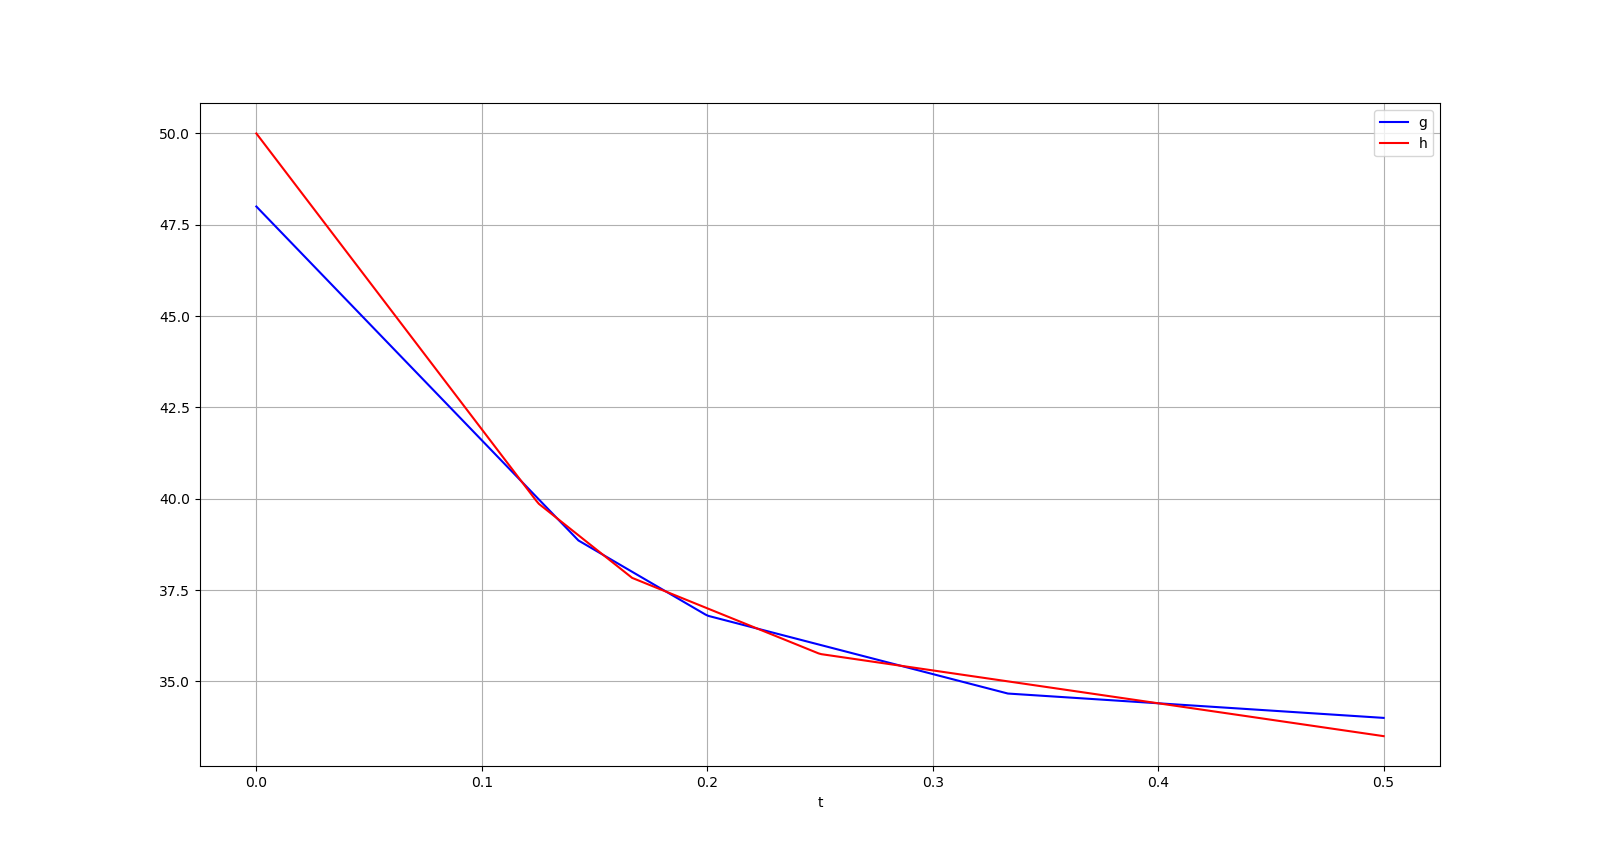
\includegraphics[scale=1, width=0.9\linewidth]{figures/chebyshev-eq-red.png}
		\caption{Example of the two functions constructed for the Chebyshev equation problem. Here the integer sequence \(1, 2, 3, 4\) was used. These functions do not change if any of the integers appear more than once. }
		\label{fig:chebyshev-eq-red}
	\end{figure}


	We define the function \(f_a(t) = C + 2a - a^2 t\) which corresponds to the maximized term on both sides without absolute value. The intuition behind this function is that \(f_a\) is the tangent on the function \(C + \frac{1}{x}\) at \(x = \frac{1}{a}\). Note that \(f_a(\frac{1}{a}) > f_b(\frac{1}{a})\) for all \(a \neq b \in \R_{> 0}\) as 
	\begin{alignat*}{3}
		& 0 &&< (b-a)^2 \\
		\iff & 0 &&> -\frac{1}{a}(b-a)^2 =  2b -\frac{b^2}{a} - a \\
		\iff & C + 2a - \frac{a^2}{a} &&> C + 2b -\frac{b^2}{a}.
	\end{alignat*}

	This means that the functions \(g(t) = \max_{i=1,\dots, d} f_{2x_i}(t)\) and \(h(t) = \max_{i=1,\dots, d} f_{2x_i+1}(t)\) consist of exactly \(d'\) many distinct line segments where \(d'\) is the amount of distinct elements as each corresponds to exactly one line segment. From \(t=0\) towards \(t = \frac{1}{2}\) all line segments are encountered in descending order of the respective \(x_i\) where the last line segment is encountered at least after \(t=1\) as we are dealing with integers and thus the maximal value of \(\frac{1}{n}\) is \(1\). 

	Note that these two functions are almost the ones from \cref{eq:red-eq-chebyshev} but without the absolute values. Thus, if all of their linear functions are positive on \([0,\frac{1}{2}]\) these two functions are equal to the sides of the equation. For \(C = \max_{i=1, \dots, d}2x_i^2\) it can be easily checked that all linear terms are positive on \([0, \frac{1}{2}]\).

	We now investigate the solutions to the equation \(g(t) = h(t)\) on \([0, \frac{1}{2}]\). For \(t = \frac{1}{2x_i}\) it holds \(g(t) > h(t)\) and for \(t = \frac{1}{2x_i + 1}\) it holds \(g(t) < h(t)\) for all \(i \in \set{1,\dots, d}\). Let \(d'\) again be the number of distinct elements. There are at least \(2d' - 1\) many solutions to the equation as there are \(2d'\) many distinct points of the form \(\frac{1}{2xi}\) and \(\frac{1}{2x_i+1}\) and the sign of \(g(t)-h(t)\) alternates between each of them. However, there cannot be more than \(2d'-1\) many solutions as each of the \(d'\) many line segments in \(g\) can only intersect at most \(2\) line segments in \(h\) because both are convex and the first and last line segment cannot both intersect \(h\) twice. Thus the amount of solutions in \([0,2]\) is exactly \(2d'-1\). 

	To decide the integer element distinctness, we construct \cref{eq:red-eq-chebyshev} and find the solutions. We iterate over them in linear time and count how many solutions there are in the interval \([0, \frac{1}{2}]\). This gives us \(2d'-1\) from which we can determine the amount of distinct elements.
\end{proof}

\begin{lemma}
	The Manhattan equation problem as stated in \cref{def:manhattan-problem} has a lower bound of \(\Omega(d \log d)\).
\end{lemma}

\begin{proof}
	Given an instance of the integer element distinctness problem \(x_1, \dots, x_d \in \N_+\). We construct the following instance of the Manhattan equation problem in \(2d\) dimensions. 
	\begin{equation}\label{eq:red-eq-manhattan}
		1 + \sum_{i=1}^d |6x_i + 4 - 2t| = \sum_{i=1}^d \parenth{|3x_i + 1 - t| + |3x_i + 3 - t|}
	\end{equation}
	
	For example instances see \cref{fig:manhattan-eq-red-1} and \cref{fig:manhattan-eq-red-2}. For a comparison of the subfunctions \(|6x_i + 4 - 2t|\) and \(|3x_i + 1 - t| + |3x_i + 3 - t|\) see \cref{fig:manhattan-building-block}.

	\begin{figure}
	  \centering
	  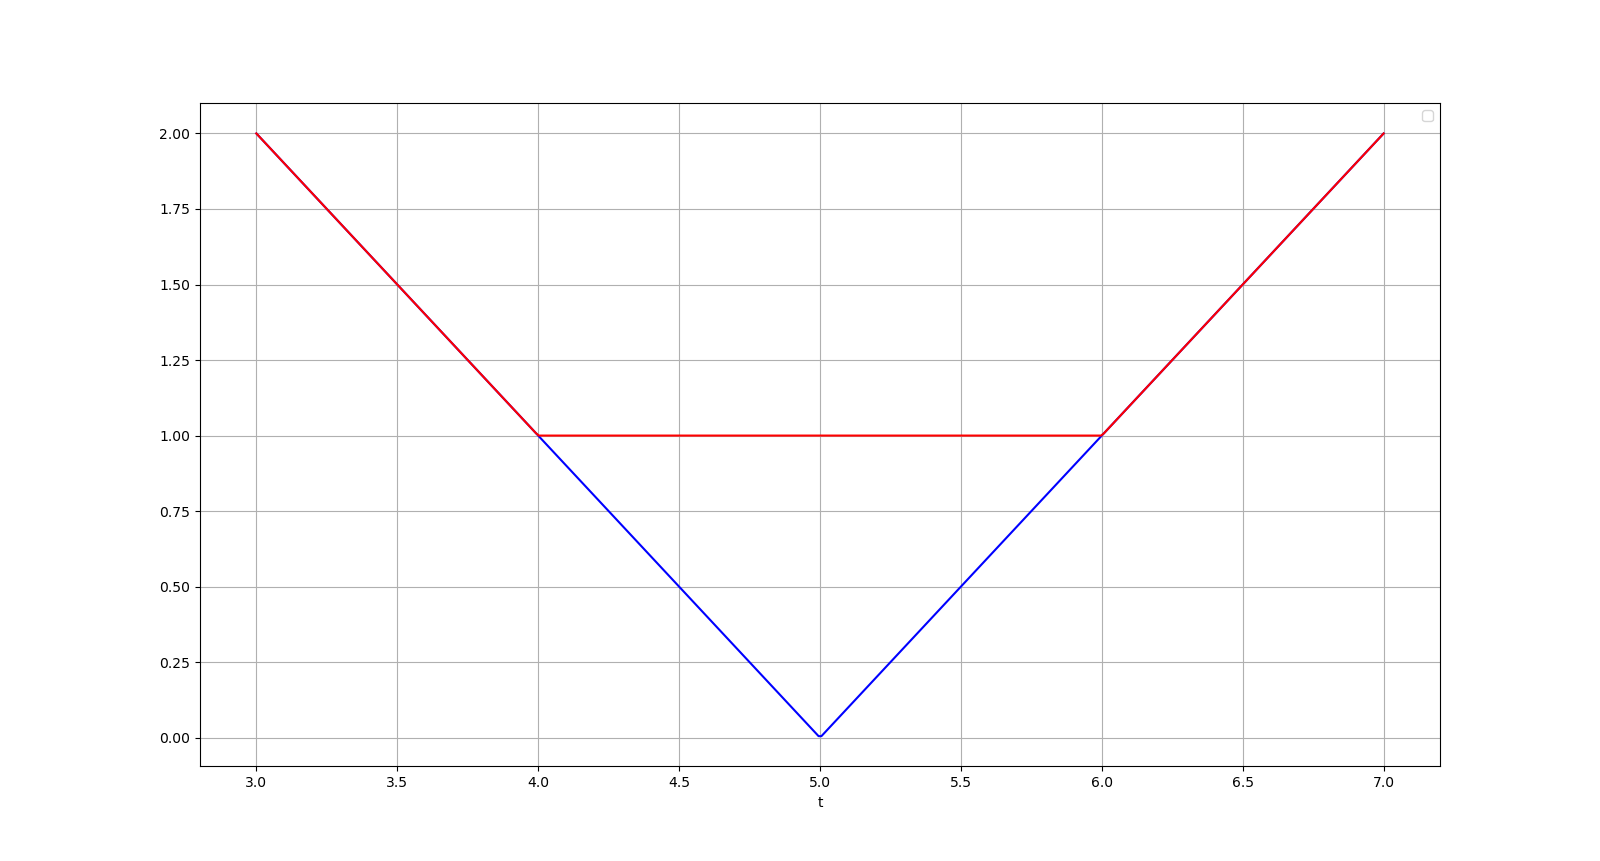
\includegraphics[scale=1, width=0.9\linewidth]{figures/manhattan-building-block.png}
	  \caption{Comparison of the functions \(|6x_i + 4 - 2t|\) and \(|3x_i + 1 - t| + |3x_i + 3 - t|\) for \(x_i = 1\).}
	  \label{fig:manhattan-building-block}
	\end{figure}

	\begin{figure}
	  \centering
	  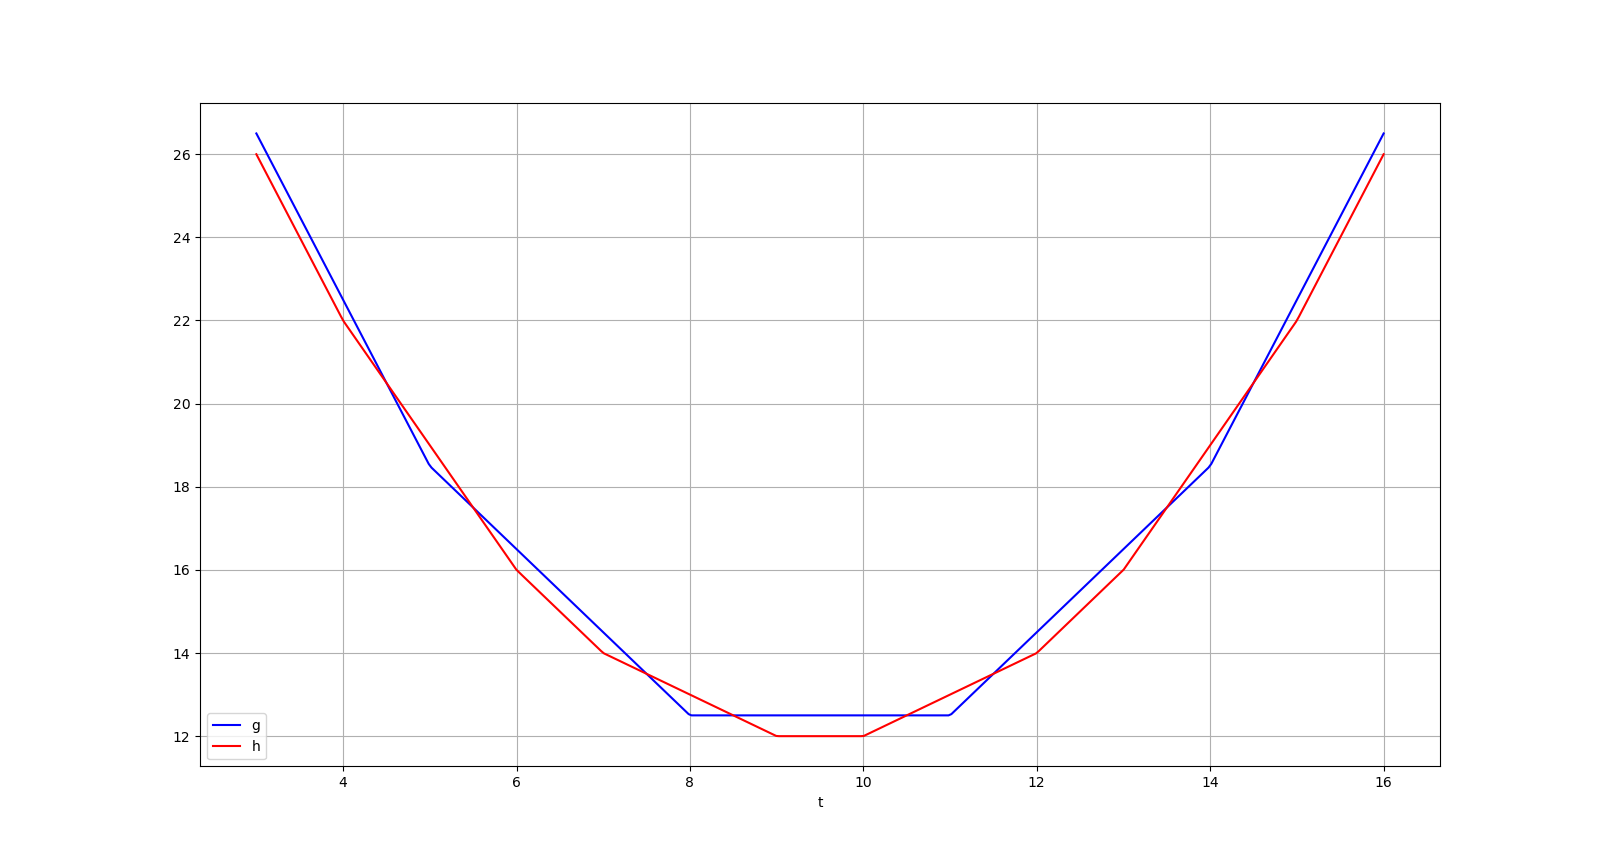
\includegraphics[scale=1, width=0.9\linewidth]{figures/manhattan-eq-red-1.png}
	  \caption{Instance for the numbers \(1,2,3,4\). There are \(8\) solutions which means there are \(4\) distinct values.}
	  \label{fig:manhattan-eq-red-1}
	\end{figure}

	\begin{figure}
	  \centering
	  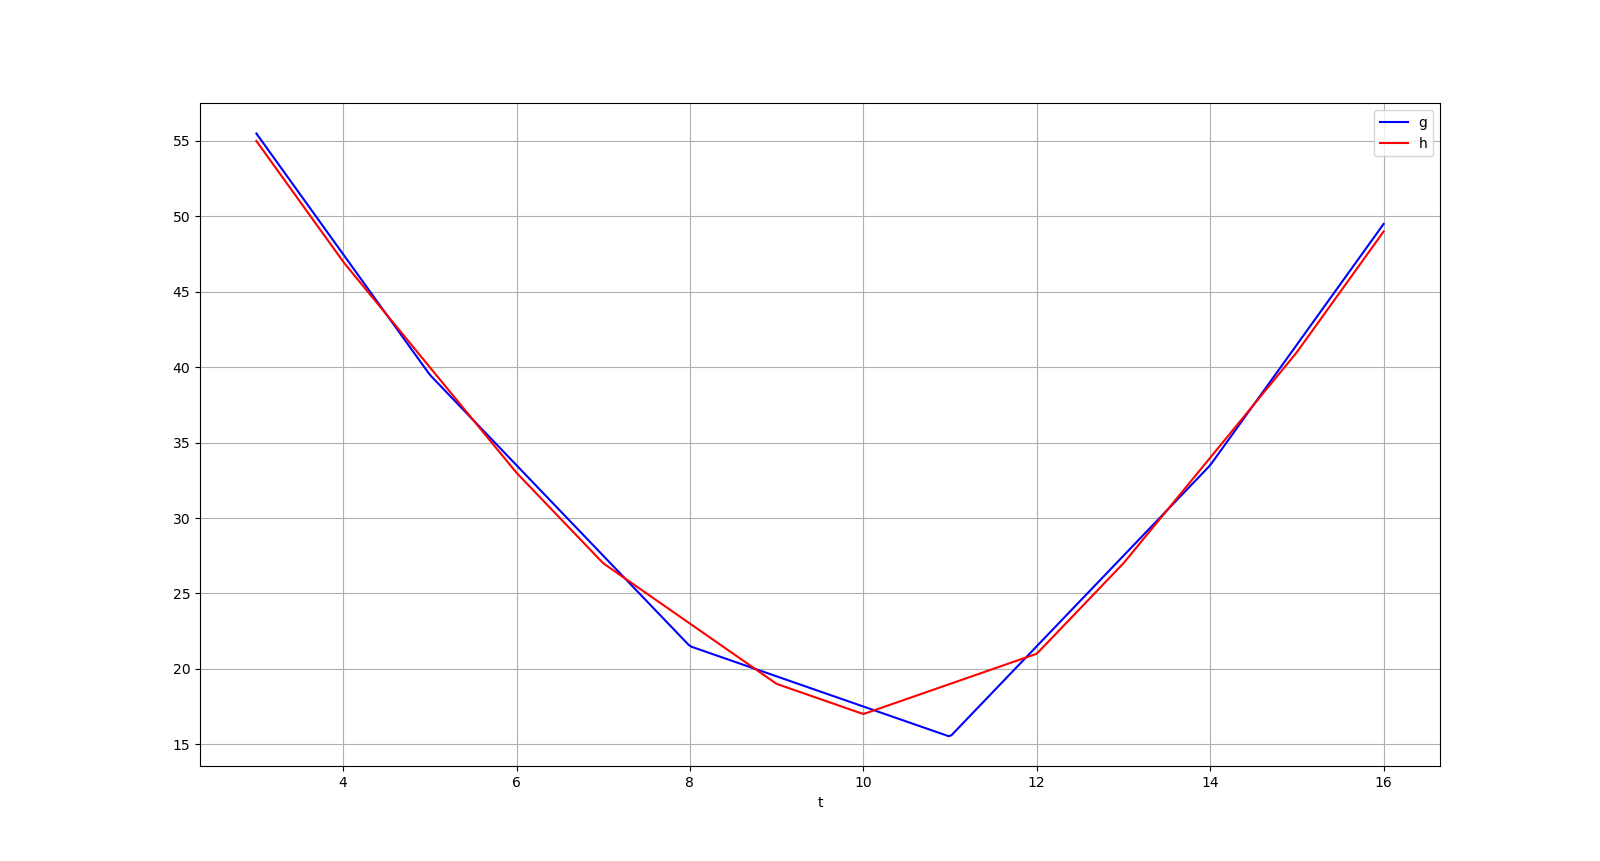
\includegraphics[scale=1, width=0.9\linewidth]{figures/manhattan-eq-red-2.png}
	  \caption{Instance for the numbers \(1,2,3,4,3,2,3,3\). The numbers \(2\) and \(3\) appear multiple times. This does not affect the amount of solutions but slightly moves their positions.}
	  \label{fig:manhattan-eq-red-2}
	\end{figure}

	It can easily be seen that for \(t \notin [3x_i + 1, 3x_i + 3]\) that \(|6x_i + 4 - 2t| = |3x_i + 1 - t| + |3x_i + 3 - t|\) and for \(t \in (3x_i + 1, 3x_i + 3)\) we get \(|6x_i + 4 - 2t| < |3x_i + 1 - t| + |3x_i + 3 - t|\). Further, the equation \(1 + k|6x_i + 4 - 2t| = k|3x_i + 1 - t| + k|3x_i + 3 - t|\) has exactly two solutions, both of which are in the interval \([3x_i+1,3x_i+3]\) for any \(k \in \N_+\). Set \(g(t) = 1 + \sum_{i=1}^d |6x_i + 4 - 2t|\) and \(h(t) = \sum_{i=1}^d \parenth{|3x_i + 1 - t| + |3x_i + 3 - t|}\).

	For \(t \in [3x_i, 3x_i + 1]\) for any \(x_i\) we can see that \(g(t) = 1 + h(t)\). For \(t \in (3x_i+1, 3x_i + 3)\) both sides of the equation are mostly the same, more specifically, \(g(t)- h(t) = 1 + k|6x_i + 4 - 2t| - k|3x_i + 1 - t| - k|3x_i + 3 - t|\) where \(k\) is the amount of datapoints which have the value \(x_i\). This has exactly two solutions in the interval. Thus the total amount of solutions is \(2d'\) where \(d'\) is the amount of distinct solutions.
\end{proof}



